\section{Developer zone: Numerical methods stage}
\label{sec: numerical_methods}
The starting point to model gas fluid dynamics is the Navier-Stokes equations with some common model simplifications used in gas pipeline networks analysis. An schematic resume of the modelling is shown in Fig. \ref{fig: scheme_model}. A complete derivation of the modelling system can be found in \cite{Cavana2020}. Here we draw only the more general key points needed for the presentation of the tool. 
\begin{figure}[H]
    \centering
    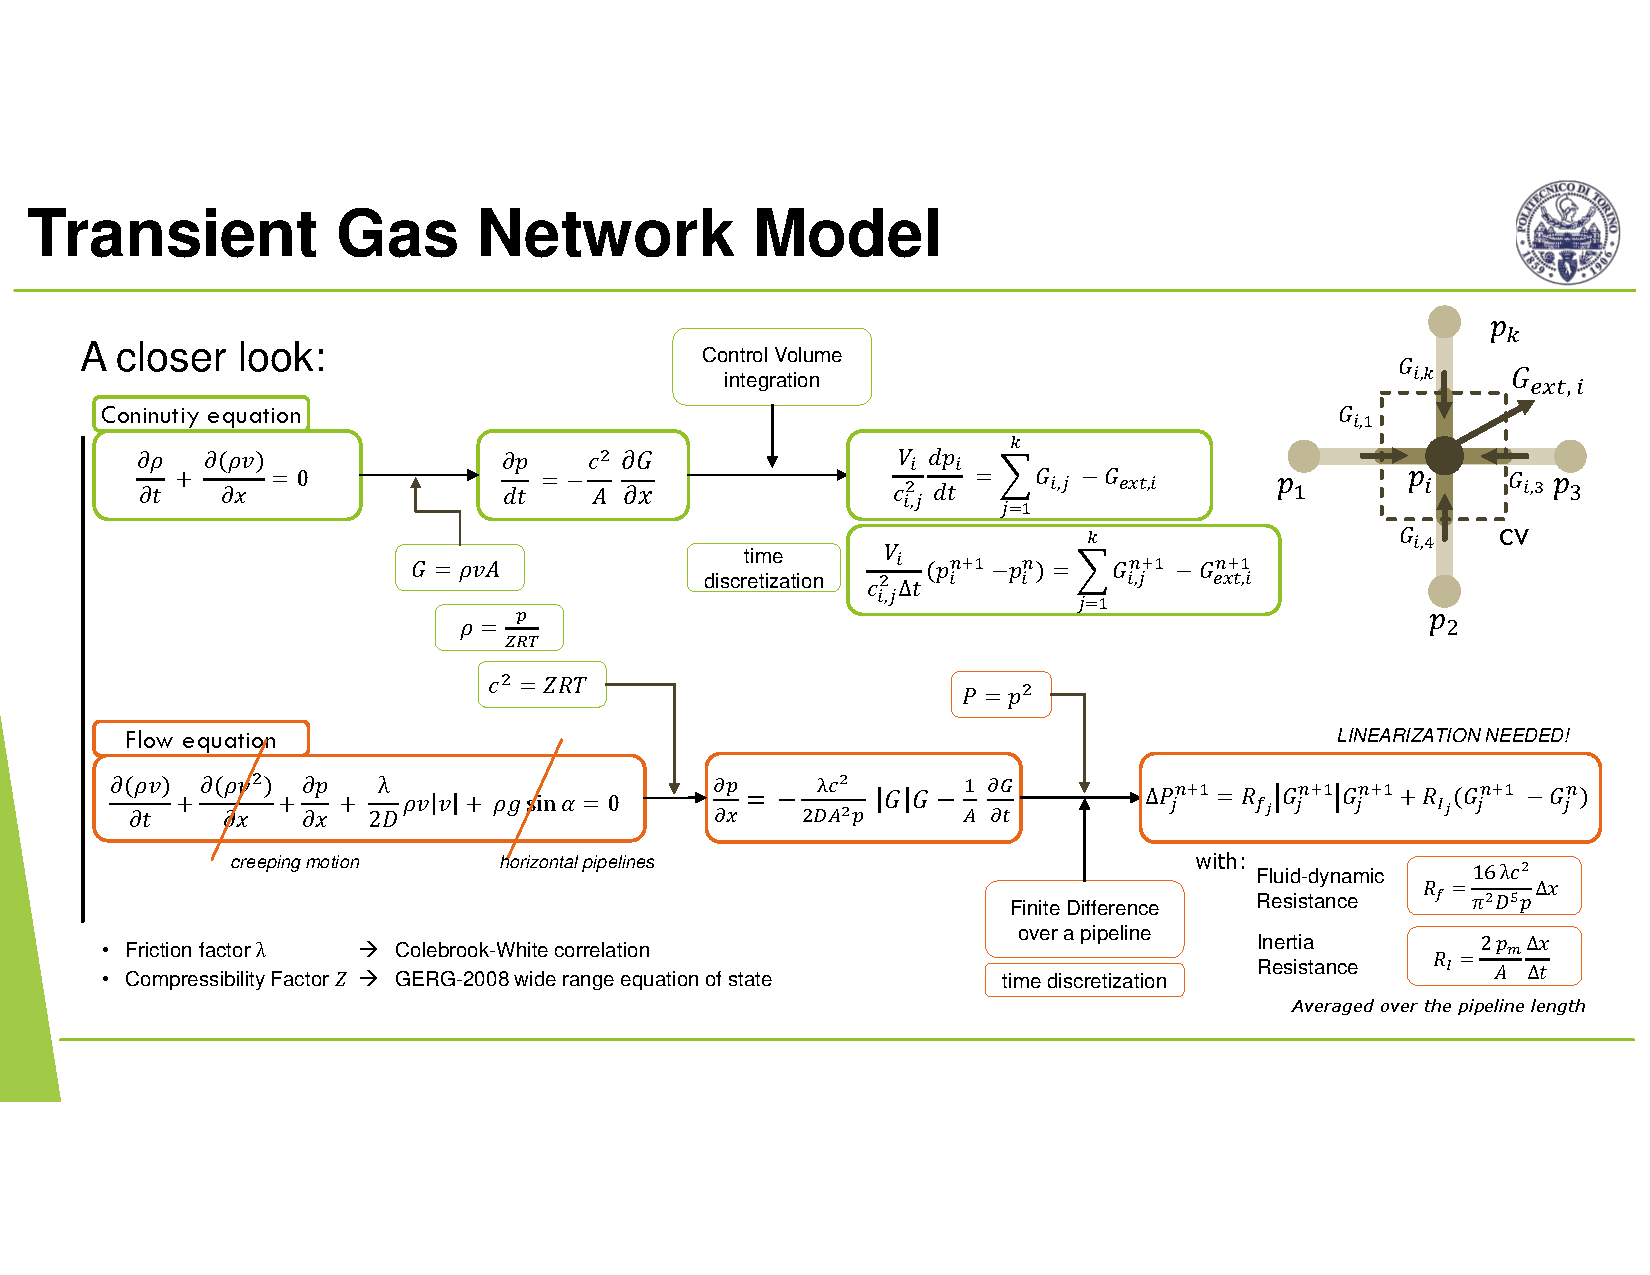
\includegraphics[scale = 0.5]{img_methods/model_scheme.pdf}
    \caption{Schematic transient gas network model.}
    \label{fig: scheme_model}
\end{figure}
The first assumption is unidimensional flow, which implies that radial variations are neglected. Another common simplification concerns long distance gas transport, which it is typically supposed to occur within an isothermal process. This assumption holds in general despite variations due to local weather, due to the stability of the soil temperature where pipelines are normally installed. Additionally, for non-isentropic processes, as such of compressors and turbines, overall this assumption seems to be a trade-off which allows avoiding to solve the energy equation. Some estimations of pressure drop error based on these assumptions are discussed in [Marco Thesis cite 92]. The second main assumption is \cred{creeping flow} \cred{[DENERG CHECK REQUIRED]}, which derives from the low Reynolds numbers mainly due to the low operational velocity of the transported gas. 
s
The structure of the methodology for the numerical methods stage can be thought as three main nested loops, shown in Fig. \ref{fig: numerical_methods_stage}. The external loop tackles the unsteady time advance, the middle loop the quality tracking and the inner loop the solution of the gas fluid dynamics.  
\begin{figure}[H]
    \centering
    % Graphic for TeX using PGF
% Title: /home/karol/Documents/UNIVERSITA/POLITO/PRESENTATIONS/SHIMMER_2024_01/img_code/numerical_methods_algorithm.dia
% Creator: Dia v0.97.3
% CreationDate: Mon Jan 22 14:41:21 2024
% For: karol
% \usepackage{tikz}
% The following commands are not supported in PSTricks at present
% We define them conditionally, so when they are implemented,
% this pgf file will use them.
\ifx\du\undefined
  \newlength{\du}
\fi
\setlength{\du}{7.5\unitlength}
\begin{tikzpicture}[even odd rule]
\pgftransformxscale{1.000000}
\pgftransformyscale{-1.000000}
\definecolor{dialinecolor}{rgb}{0.000000, 0.000000, 0.000000}
\pgfsetstrokecolor{dialinecolor}
\pgfsetstrokeopacity{1.000000}
\definecolor{diafillcolor}{rgb}{1.000000, 1.000000, 1.000000}
\pgfsetfillcolor{diafillcolor}
\pgfsetfillopacity{1.000000}
\pgfsetlinewidth{0.100000\du}
\pgfsetdash{{\pgflinewidth}{0.200000\du}}{0cm}
\pgfsetmiterjoin
\pgfsetbuttcap
{
%\pgfsetcornersarced{\pgfpoint{0.000000\du}{0.000000\du}}\definecolor{diafillcolor}{rgb}{0.898039, 0.898039, 0.898039}
\pgfsetcornersarced{\pgfpoint{0.000000\du}{0.000000\du}}
\pgfsetfillcolor{lgreyblue}
\pgfsetfillopacity{1.000000}
\fill (5.263771\du,-6.474566\du)--(5.263771\du,15.452514\du)--(19.576450\du,15.452514\du)--(19.576450\du,-6.474566\du)--cycle;
}{\pgfsetcornersarced{\pgfpoint{0.000000\du}{0.000000\du}}\definecolor{dialinecolor}{rgb}{0.000000, 0.000000, 0.000000}
% Time stroke
\only<1-2>{\pgfsetstrokecolor{diafillcolor}}
\only<3->{\pgfsetstrokecolor{red}}

\pgfsetstrokeopacity{1.000000}
\draw (5.263771\du,-6.474566\du)--(5.263771\du,15.452514\du)--(19.576450\du,15.452514\du)--(19.576450\du,-6.474566\du)--cycle;
}\pgfsetlinewidth{0.100000\du}
\pgfsetdash{{\pgflinewidth}{0.200000\du}}{0cm}
\pgfsetmiterjoin
\pgfsetbuttcap
{\pgfsetcornersarced{\pgfpoint{0.000000\du}{0.000000\du}}\definecolor{diafillcolor}{rgb}{0.945098, 0.882353, 0.921569}
\pgfsetfillcolor{diafillcolor}
\pgfsetfillopacity{1.000000}
\fill (6.382560\du,-3.393932\du)--(6.382560\du,10.487096\du)--(17.858929\du,10.487096\du)--(17.858929\du,-3.393932\du)--cycle;
}{\pgfsetcornersarced{\pgfpoint{0.000000\du}{0.000000\du}}\definecolor{dialinecolor}{rgb}{0.403922, 0.047059, 0.274510}
\only<1>{\pgfsetstrokecolor{dialinecolor}}
\only<2->{\pgfsetstrokecolor{red}}
\pgfsetstrokeopacity{1.000000}
\draw (6.382560\du,-3.393932\du)--(6.382560\du,10.487096\du)--(17.858929\du,10.487096\du)--(17.858929\du,-3.393932\du)--cycle;
}\pgfsetlinewidth{0.100000\du}
\pgfsetdash{{\pgflinewidth}{0.200000\du}}{0cm}
\pgfsetmiterjoin
\pgfsetbuttcap
{\pgfsetcornersarced{\pgfpoint{0.000000\du}{0.000000\du}}\definecolor{diafillcolor}{rgb}{0.847059, 0.898039, 0.898039}
\pgfsetfillcolor{diafillcolor}
\pgfsetfillopacity{1.000000}
\fill (7.111444\du,-0.032868\du)--(7.111444\du,7.295393\du)--(13.953260\du,7.295393\du)--(13.953260\du,-0.032868\du)--cycle;
}{\pgfsetcornersarced{\pgfpoint{0.000000\du}{0.000000\du}}\definecolor{dialinecolor}{rgb}{0.003876, 0.318700, 0.318700}
\pgfsetstrokecolor{dialinecolor}
\pgfsetstrokeopacity{1.000000}
\draw (7.111444\du,-0.032868\du)--(7.111444\du,7.295393\du)--(13.953260\du,7.295393\du)--(13.953260\du,-0.032868\du)--cycle;
}\pgfsetlinewidth{0.100000\du}
\pgfsetdash{}{0pt}
\pgfsetbuttcap
\pgfsetmiterjoin
\pgfsetlinewidth{0.100000\du}
\pgfsetbuttcap
\pgfsetmiterjoin
\pgfsetdash{}{0pt}
\definecolor{diafillcolor}{rgb}{1.000000, 1.000000, 1.000000}
\pgfsetfillcolor{diafillcolor}
\pgfsetfillopacity{1.000000}
\definecolor{dialinecolor}{rgb}{0.000000, 0.000000, 0.000000}
\pgfsetstrokecolor{dialinecolor}
\pgfsetstrokeopacity{1.000000}
\pgfpathmoveto{\pgfpoint{8.300000\du}{0.200000\du}}
\pgfpathlineto{\pgfpoint{9.900000\du}{0.200000\du}}
\pgfpathcurveto{\pgfpoint{10.120914\du}{0.200000\du}}{\pgfpoint{10.300000\du}{0.401472\du}}{\pgfpoint{10.300000\du}{0.650000\du}}
\pgfpathcurveto{\pgfpoint{10.300000\du}{0.898528\du}}{\pgfpoint{10.120914\du}{1.100000\du}}{\pgfpoint{9.900000\du}{1.100000\du}}
\pgfpathlineto{\pgfpoint{8.300000\du}{1.100000\du}}
\pgfpathcurveto{\pgfpoint{8.079086\du}{1.100000\du}}{\pgfpoint{7.900000\du}{0.898528\du}}{\pgfpoint{7.900000\du}{0.650000\du}}
\pgfpathcurveto{\pgfpoint{7.900000\du}{0.401472\du}}{\pgfpoint{8.079086\du}{0.200000\du}}{\pgfpoint{8.300000\du}{0.200000\du}}
\pgfpathclose
\pgfusepath{fill,stroke}
% setfont left to latex
% setfont left to latex
\definecolor{dialinecolor}{rgb}{0.000000, 0.000000, 0.000000}
\pgfsetstrokecolor{dialinecolor}
\pgfsetstrokeopacity{1.000000}
\definecolor{diafillcolor}{rgb}{0.000000, 0.000000, 0.000000}
\pgfsetfillcolor{diafillcolor}
\pgfsetfillopacity{1.000000}
\node[anchor=base,inner sep=0pt, outer sep=0pt,color=dialinecolor] at (9.100000\du,0.950000\du){};
\pgfsetlinewidth{0.100000\du}
\pgfsetdash{}{0pt}
\pgfsetbuttcap
{
\definecolor{diafillcolor}{rgb}{0.000000, 0.000000, 0.000000}
\pgfsetfillcolor{diafillcolor}
\pgfsetfillopacity{1.000000}
% was here!!!
\definecolor{dialinecolor}{rgb}{0.000000, 0.000000, 0.000000}
\pgfsetstrokecolor{dialinecolor}
\pgfsetstrokeopacity{1.000000}
\draw (9.100000\du,1.100000\du)--(9.100000\du,1.550000\du);
}
\pgfsetlinewidth{0.100000\du}
\pgfsetdash{}{0pt}
\pgfsetmiterjoin
{\pgfsetcornersarced{\pgfpoint{0.000000\du}{0.000000\du}}\definecolor{diafillcolor}{rgb}{1.000000, 1.000000, 1.000000}
\pgfsetfillcolor{diafillcolor}
\pgfsetfillopacity{1.000000}
\fill (7.600000\du,1.550000\du)--(7.600000\du,2.323485\du)--(10.600000\du,2.323485\du)--(10.600000\du,1.550000\du)--cycle;
}{\pgfsetcornersarced{\pgfpoint{0.000000\du}{0.000000\du}}\definecolor{dialinecolor}{rgb}{0.000000, 0.000000, 0.000000}
\pgfsetstrokecolor{dialinecolor}
\pgfsetstrokeopacity{1.000000}
\draw (7.600000\du,1.550000\du)--(7.600000\du,2.323485\du)--(10.600000\du,2.323485\du)--(10.600000\du,1.550000\du)--cycle;
}% setfont left to latex
% setfont left to latex
\definecolor{dialinecolor}{rgb}{0.000000, 0.000000, 0.000000}
\pgfsetstrokecolor{dialinecolor}
\pgfsetstrokeopacity{1.000000}
\definecolor{diafillcolor}{rgb}{0.000000, 0.000000, 0.000000}
\pgfsetfillcolor{diafillcolor}
\pgfsetfillopacity{1.000000}
\node[anchor=base,inner sep=0pt, outer sep=0pt,color=dialinecolor] at (9.100000\du,2.191526\du){};
\pgfsetlinewidth{0.100000\du}
\pgfsetdash{}{0pt}
\pgfsetmiterjoin
\definecolor{diafillcolor}{rgb}{1.000000, 1.000000, 1.000000}
\pgfsetfillcolor{diafillcolor}
\pgfsetfillopacity{1.000000}
\fill (9.099017\du,2.996875\du)--(10.616784\du,3.496875\du)--(9.099017\du,3.996875\du)--(7.581250\du,3.496875\du)--cycle;
\definecolor{dialinecolor}{rgb}{0.000000, 0.000000, 0.000000}
\pgfsetstrokecolor{dialinecolor}
\pgfsetstrokeopacity{1.000000}
\draw (9.099017\du,2.996875\du)--(10.616784\du,3.496875\du)--(9.099017\du,3.996875\du)--(7.581250\du,3.496875\du)--cycle;
% setfont left to latex
% setfont left to latex
\definecolor{dialinecolor}{rgb}{0.000000, 0.000000, 0.000000}
\pgfsetstrokecolor{dialinecolor}
\pgfsetstrokeopacity{1.000000}
\definecolor{diafillcolor}{rgb}{0.000000, 0.000000, 0.000000}
\pgfsetfillcolor{diafillcolor}
\pgfsetfillopacity{1.000000}
\node[anchor=base,inner sep=0pt, outer sep=0pt,color=dialinecolor] at (9.099017\du,3.781875\du){};
\pgfsetlinewidth{0.100000\du}
\pgfsetdash{}{0pt}
\pgfsetbuttcap
{
\definecolor{diafillcolor}{rgb}{0.000000, 0.000000, 0.000000}
\pgfsetfillcolor{diafillcolor}
\pgfsetfillopacity{1.000000}
% was here!!!
\definecolor{dialinecolor}{rgb}{0.000000, 0.000000, 0.000000}
\pgfsetstrokecolor{dialinecolor}
\pgfsetstrokeopacity{1.000000}
\draw (9.099017\du,3.996875\du)--(9.102774\du,4.529549\du);
}
\pgfsetlinewidth{0.100000\du}
\pgfsetdash{}{0pt}
\pgfsetmiterjoin
{\pgfsetcornersarced{\pgfpoint{0.000000\du}{0.000000\du}}\definecolor{diafillcolor}{rgb}{1.000000, 1.000000, 1.000000}
\pgfsetfillcolor{diafillcolor}
\pgfsetfillopacity{1.000000}
\fill (7.602774\du,4.529549\du)--(7.602774\du,5.346335\du)--(10.602774\du,5.346335\du)--(10.602774\du,4.529549\du)--cycle;
}{\pgfsetcornersarced{\pgfpoint{0.000000\du}{0.000000\du}}\definecolor{dialinecolor}{rgb}{0.000000, 0.000000, 0.000000}
\pgfsetstrokecolor{dialinecolor}
\pgfsetstrokeopacity{1.000000}
\draw (7.602774\du,4.529549\du)--(7.602774\du,5.346335\du)--(10.602774\du,5.346335\du)--(10.602774\du,4.529549\du)--cycle;
}% setfont left to latex
% setfont left to latex
\definecolor{dialinecolor}{rgb}{0.000000, 0.000000, 0.000000}
\pgfsetstrokecolor{dialinecolor}
\pgfsetstrokeopacity{1.000000}
\definecolor{diafillcolor}{rgb}{0.000000, 0.000000, 0.000000}
\pgfsetfillcolor{diafillcolor}
\pgfsetfillopacity{1.000000}
\node[anchor=base,inner sep=0pt, outer sep=0pt,color=dialinecolor] at (9.102774\du,5.192725\du){};
\pgfsetlinewidth{0.100000\du}
\pgfsetdash{}{0pt}
\pgfsetbuttcap
{
\definecolor{diafillcolor}{rgb}{0.000000, 0.000000, 0.000000}
\pgfsetfillcolor{diafillcolor}
\pgfsetfillopacity{1.000000}
% was here!!!
\definecolor{dialinecolor}{rgb}{0.000000, 0.000000, 0.000000}
\pgfsetstrokecolor{dialinecolor}
\pgfsetstrokeopacity{1.000000}
\draw (9.100000\du,2.323485\du)--(9.099017\du,2.996875\du);
}
\pgfsetlinewidth{0.100000\du}
\pgfsetdash{}{0pt}
\pgfsetbuttcap
{
\definecolor{diafillcolor}{rgb}{0.000000, 0.000000, 0.000000}
\pgfsetfillcolor{diafillcolor}
\pgfsetfillopacity{1.000000}
% was here!!!
\definecolor{dialinecolor}{rgb}{0.000000, 0.000000, 0.000000}
\pgfsetstrokecolor{dialinecolor}
\pgfsetstrokeopacity{1.000000}
\draw (10.616784\du,3.496875\du)--(11.080431\du,3.494330\du);
}
\pgfsetlinewidth{0.100000\du}
\pgfsetdash{}{0pt}
\pgfsetmiterjoin
{\pgfsetcornersarced{\pgfpoint{0.000000\du}{0.000000\du}}\definecolor{diafillcolor}{rgb}{1.000000, 1.000000, 1.000000}
\pgfsetfillcolor{diafillcolor}
\pgfsetfillopacity{1.000000}
\fill (11.080431\du,3.085936\du)--(11.080431\du,3.902723\du)--(13.643775\du,3.902723\du)--(13.643775\du,3.085936\du)--cycle;
}{\pgfsetcornersarced{\pgfpoint{0.000000\du}{0.000000\du}}\definecolor{dialinecolor}{rgb}{0.000000, 0.000000, 0.000000}
\pgfsetstrokecolor{dialinecolor}
\pgfsetstrokeopacity{1.000000}
\draw (11.080431\du,3.085936\du)--(11.080431\du,3.902723\du)--(13.643775\du,3.902723\du)--(13.643775\du,3.085936\du)--cycle;
}% setfont left to latex
% setfont left to latex
\definecolor{dialinecolor}{rgb}{0.000000, 0.000000, 0.000000}
\pgfsetstrokecolor{dialinecolor}
\pgfsetstrokeopacity{1.000000}
\definecolor{diafillcolor}{rgb}{0.000000, 0.000000, 0.000000}
\pgfsetfillcolor{diafillcolor}
\pgfsetfillopacity{1.000000}
\node[anchor=base,inner sep=0pt, outer sep=0pt,color=dialinecolor] at (12.362103\du,3.749113\du){};
\pgfsetlinewidth{0.100000\du}
\pgfsetdash{}{0pt}
\pgfsetmiterjoin
\pgfsetbuttcap
{
\definecolor{diafillcolor}{rgb}{0.000000, 0.000000, 0.000000}
\pgfsetfillcolor{diafillcolor}
\pgfsetfillopacity{1.000000}
% was here!!!
{\pgfsetcornersarced{\pgfpoint{0.000000\du}{0.000000\du}}\definecolor{dialinecolor}{rgb}{0.000000, 0.000000, 0.000000}
\pgfsetstrokecolor{dialinecolor}
\pgfsetstrokeopacity{1.000000}
\draw (10.602774\du,5.142139\du)--(12.362103\du,5.142139\du)--(12.362103\du,3.902723\du);
}}
\pgfsetlinewidth{0.100000\du}
\pgfsetdash{}{0pt}
\pgfsetbuttcap
\pgfsetmiterjoin
\pgfsetlinewidth{0.100000\du}
\pgfsetbuttcap
\pgfsetmiterjoin
\pgfsetdash{}{0pt}
\definecolor{diafillcolor}{rgb}{1.000000, 1.000000, 1.000000}
\pgfsetfillcolor{diafillcolor}
\pgfsetfillopacity{1.000000}
\definecolor{dialinecolor}{rgb}{0.000000, 0.000000, 0.000000}
\pgfsetstrokecolor{dialinecolor}
\pgfsetstrokeopacity{1.000000}
\pgfpathmoveto{\pgfpoint{8.304290\du}{5.979312\du}}
\pgfpathlineto{\pgfpoint{9.904290\du}{5.979312\du}}
\pgfpathcurveto{\pgfpoint{10.125204\du}{5.979312\du}}{\pgfpoint{10.304290\du}{6.180783\du}}{\pgfpoint{10.304290\du}{6.429312\du}}
\pgfpathcurveto{\pgfpoint{10.304290\du}{6.677840\du}}{\pgfpoint{10.125204\du}{6.879312\du}}{\pgfpoint{9.904290\du}{6.879312\du}}
\pgfpathlineto{\pgfpoint{8.304290\du}{6.879312\du}}
\pgfpathcurveto{\pgfpoint{8.083376\du}{6.879312\du}}{\pgfpoint{7.904290\du}{6.677840\du}}{\pgfpoint{7.904290\du}{6.429312\du}}
\pgfpathcurveto{\pgfpoint{7.904290\du}{6.180783\du}}{\pgfpoint{8.083376\du}{5.979312\du}}{\pgfpoint{8.304290\du}{5.979312\du}}
\pgfpathclose
\pgfusepath{fill,stroke}
% setfont left to latex
% setfont left to latex
\definecolor{dialinecolor}{rgb}{0.000000, 0.000000, 0.000000}
\pgfsetstrokecolor{dialinecolor}
\pgfsetstrokeopacity{1.000000}
\definecolor{diafillcolor}{rgb}{0.000000, 0.000000, 0.000000}
\pgfsetfillcolor{diafillcolor}
\pgfsetfillopacity{1.000000}
\node[anchor=base,inner sep=0pt, outer sep=0pt,color=dialinecolor] at (9.104290\du,6.729312\du){};
\pgfsetlinewidth{0.100000\du}
\pgfsetdash{}{0pt}
\pgfsetbuttcap
{
\definecolor{diafillcolor}{rgb}{0.000000, 0.000000, 0.000000}
\pgfsetfillcolor{diafillcolor}
\pgfsetfillopacity{1.000000}
% was here!!!
\definecolor{dialinecolor}{rgb}{0.000000, 0.000000, 0.000000}
\pgfsetstrokecolor{dialinecolor}
\pgfsetstrokeopacity{1.000000}
\draw (9.102774\du,5.346335\du)--(9.104290\du,5.979312\du);
}
% setfont left to latex
% setfont left to latex
\definecolor{dialinecolor}{rgb}{0.000000, 0.000000, 0.000000}
\pgfsetstrokecolor{dialinecolor}
\pgfsetstrokeopacity{1.000000}
\definecolor{diafillcolor}{rgb}{0.000000, 0.000000, 0.000000}
\pgfsetfillcolor{diafillcolor}
\pgfsetfillopacity{1.000000}
\node[anchor=base west,inner sep=0pt,outer sep=0pt,color=dialinecolor] at (11.506559\du,-0.738088\du){};
% setfont left to latex
% setfont left to latex

\pgfsetstrokecolor{dialinecolor}
\pgfsetstrokeopacity{1.000000}
\pgfsetfillcolor{diafillcolor}
\pgfsetfillopacity{1.000000}
\node[anchor=base west,inner sep=0pt,outer sep=0pt,color=tealgreen] at (11.5\du,0.8 \du){\scriptsize {\textbf{Fluid}}};
\node[anchor=base west,inner sep=0pt,outer sep=0pt,color=tealgreen] at (11.5\du,1.55\du){\scriptsize {\textbf{solver}}};


\definecolor{dialinecolor}{rgb}{0.000000, 0.317647, 0.317647}
\pgfsetstrokecolor{dialinecolor}
\pgfsetstrokeopacity{1.000000}
\definecolor{diafillcolor}{rgb}{0.000000, 0.317647, 0.317647}
\pgfsetfillcolor{red}
\pgfsetfillopacity{1.000000}
% setfont left to latex
% setfont left to latex
\definecolor{dialinecolor}{rgb}{0.000000, 0.317647, 0.317647}
\pgfsetstrokecolor{dialinecolor}
\pgfsetstrokeopacity{1.000000}
\definecolor{diafillcolor}{rgb}{0.000000, 0.317647, 0.317647}
\pgfsetfillcolor{red}
\pgfsetfillopacity{1.000000}
\node[anchor=base west,inner sep=0pt,outer sep=0pt,color=dialinecolor] at (11.178222\du,1.315313\du){};
% setfont left to latex
% setfont left to latex
\definecolor{dialinecolor}{rgb}{0.000000, 0.000000, 0.000000}
\pgfsetstrokecolor{dialinecolor}
\pgfsetstrokeopacity{1.000000}
\definecolor{diafillcolor}{rgb}{0.000000, 0.000000, 0.000000}
\pgfsetfillcolor{diafillcolor}
\pgfsetfillopacity{1.000000}
\node[anchor=base west,inner sep=0pt,outer sep=0pt,color=dialinecolor] at (9.691002\du,-1.143346\du){};
% setfont left to latex
% setfont left to latex
\definecolor{dialinecolor}{rgb}{0.000000, 0.000000, 0.000000}
\pgfsetstrokecolor{dialinecolor}
\pgfsetstrokeopacity{1.000000}
\definecolor{diafillcolor}{rgb}{0.000000, 0.000000, 0.000000}
\pgfsetfillcolor{diafillcolor}
\pgfsetfillopacity{1.000000}
\node[anchor=base west,inner sep=0pt,outer sep=0pt,color=dialinecolor] at (9.766373\du,10.513799\du){};
% setfont left to latex
% setfont left to latex

\pgfsetstrokecolor{red}
\pgfsetstrokeopacity{1.000000}

\only<1>{\node[anchor=base west,inner sep=0pt,outer sep=0pt,color=vinotinto] at (11\du,-1.5\du){\scriptsize \textbf{Quality cycle}}};
\only<2->{\node[anchor=base west,inner sep=0pt,outer sep=0pt,color=red] at (11\du,-1.5\du){\scriptsize \textbf{Quality cycle}};}
\pgfsetlinewidth{0.100000\du}
\pgfsetdash{}{0pt}
\pgfsetbuttcap
{
\definecolor{diafillcolor}{rgb}{0.000000, 0.000000, 0.000000}
\pgfsetfillcolor{diafillcolor}
\pgfsetfillopacity{1.000000}
% was here!!!
\definecolor{dialinecolor}{rgb}{0.000000, 0.000000, 0.000000}
\pgfsetstrokecolor{dialinecolor}
\pgfsetstrokeopacity{1.000000}
\draw (9.099526\du,6.929167\du)--(9.090757\du,7.849149\du);
}
\pgfsetlinewidth{0.100000\du}
\pgfsetdash{}{0pt}
\pgfsetmiterjoin
{\pgfsetcornersarced{\pgfpoint{0.000000\du}{0.000000\du}}\definecolor{diafillcolor}{rgb}{1.000000, 1.000000, 1.000000}
\pgfsetfillcolor{diafillcolor}
\pgfsetfillopacity{1.000000}
\fill (7.590757\du,7.849149\du)--(7.590757\du,8.622634\du)--(10.590757\du,8.622634\du)--(10.590757\du,7.849149\du)--cycle;
}{\pgfsetcornersarced{\pgfpoint{0.000000\du}{0.000000\du}}\definecolor{dialinecolor}{rgb}{0.000000, 0.000000, 0.000000}
\pgfsetstrokecolor{dialinecolor}
\pgfsetstrokeopacity{1.000000}
\draw (7.590757\du,7.849149\du)--(7.590757\du,8.622634\du)--(10.590757\du,8.622634\du)--(10.590757\du,7.849149\du)--cycle;
}% setfont left to latex
% setfont left to latex
\definecolor{dialinecolor}{rgb}{0.000000, 0.000000, 0.000000}
\pgfsetstrokecolor{dialinecolor}
\pgfsetstrokeopacity{1.000000}
\definecolor{diafillcolor}{rgb}{0.000000, 0.000000, 0.000000}
\pgfsetfillcolor{diafillcolor}
\pgfsetfillopacity{1.000000}
\node[anchor=base,inner sep=0pt, outer sep=0pt,color=dialinecolor] at (9.090757\du,8.490675\du){};
\pgfsetlinewidth{0.100000\du}
\pgfsetdash{}{0pt}
\pgfsetmiterjoin
\definecolor{diafillcolor}{rgb}{1.000000, 1.000000, 1.000000}
\pgfsetfillcolor{diafillcolor}
\pgfsetfillopacity{1.000000}
\fill (9.089775\du,8.996139\du)--(10.607542\du,9.496139\du)--(9.089775\du,9.996139\du)--(7.572008\du,9.496139\du)--cycle;
\definecolor{dialinecolor}{rgb}{0.000000, 0.000000, 0.000000}
\pgfsetstrokecolor{dialinecolor}
\pgfsetstrokeopacity{1.000000}
\draw (9.089775\du,8.996139\du)--(10.607542\du,9.496139\du)--(9.089775\du,9.996139\du)--(7.572008\du,9.496139\du)--cycle;
% setfont left to latex
% setfont left to latex
\definecolor{dialinecolor}{rgb}{0.000000, 0.000000, 0.000000}
\pgfsetstrokecolor{dialinecolor}
\pgfsetstrokeopacity{1.000000}
\definecolor{diafillcolor}{rgb}{0.000000, 0.000000, 0.000000}
\pgfsetfillcolor{diafillcolor}
\pgfsetfillopacity{1.000000}
\node[anchor=base,inner sep=0pt, outer sep=0pt,color=dialinecolor] at (9.089775\du,9.781139\du){};
\pgfsetlinewidth{0.100000\du}
\pgfsetdash{}{0pt}
\pgfsetbuttcap
{
\definecolor{diafillcolor}{rgb}{0.000000, 0.000000, 0.000000}
\pgfsetfillcolor{diafillcolor}
\pgfsetfillopacity{1.000000}
% was here!!!
\definecolor{dialinecolor}{rgb}{0.000000, 0.000000, 0.000000}
\pgfsetstrokecolor{dialinecolor}
\pgfsetstrokeopacity{1.000000}
\draw (9.090757\du,8.622634\du)--(9.089775\du,8.996139\du);
}
\pgfsetlinewidth{0.100000\du}
\pgfsetdash{}{0pt}
\pgfsetmiterjoin
{\pgfsetcornersarced{\pgfpoint{0.000000\du}{0.000000\du}}\definecolor{diafillcolor}{rgb}{1.000000, 1.000000, 1.000000}
\pgfsetfillcolor{diafillcolor}
\pgfsetfillopacity{1.000000}
\fill (14.966081\du,7.491214\du)--(14.966081\du,8.308000\du)--(17.529425\du,8.308000\du)--(17.529425\du,7.491214\du)--cycle;
}{\pgfsetcornersarced{\pgfpoint{0.000000\du}{0.000000\du}}\definecolor{dialinecolor}{rgb}{0.000000, 0.000000, 0.000000}
\pgfsetstrokecolor{dialinecolor}
\pgfsetstrokeopacity{1.000000}
\draw (14.966081\du,7.491214\du)--(14.966081\du,8.308000\du)--(17.529425\du,8.308000\du)--(17.529425\du,7.491214\du)--cycle;
}% setfont left to latex
% setfont left to latex
\definecolor{dialinecolor}{rgb}{0.000000, 0.000000, 0.000000}
\pgfsetstrokecolor{dialinecolor}
\pgfsetstrokeopacity{1.000000}
\definecolor{diafillcolor}{rgb}{0.000000, 0.000000, 0.000000}
\pgfsetfillcolor{diafillcolor}
\pgfsetfillopacity{1.000000}
\node[anchor=base,inner sep=0pt, outer sep=0pt,color=dialinecolor] at (16.247753\du,8.154390\du){};
\pgfsetlinewidth{0.100000\du}
\pgfsetdash{}{0pt}
\pgfsetmiterjoin
\pgfsetbuttcap
{
\definecolor{diafillcolor}{rgb}{0.000000, 0.000000, 0.000000}
\pgfsetfillcolor{diafillcolor}
\pgfsetfillopacity{1.000000}
% was here!!!
{\pgfsetcornersarced{\pgfpoint{0.000000\du}{0.000000\du}}\definecolor{dialinecolor}{rgb}{0.000000, 0.000000, 0.000000}
\pgfsetstrokecolor{dialinecolor}
\pgfsetstrokeopacity{1.000000}
\draw (10.607542\du,9.496139\du)--(16.250456\du,9.496139\du)--(16.250456\du,8.308000\du)--(16.247753\du,8.308000\du);
}}
\pgfsetlinewidth{0.100000\du}
\pgfsetdash{}{0pt}
\pgfsetmiterjoin
\pgfsetbuttcap
{
\definecolor{diafillcolor}{rgb}{0.000000, 0.000000, 0.000000}
\pgfsetfillcolor{diafillcolor}
\pgfsetfillopacity{1.000000}
% was here!!!
{\pgfsetcornersarced{\pgfpoint{0.000000\du}{0.000000\du}}\definecolor{dialinecolor}{rgb}{0.000000, 0.000000, 0.000000}
\pgfsetstrokecolor{dialinecolor}
\pgfsetstrokeopacity{1.000000}
\draw (16.247753\du,7.491214\du)--(16.247753\du,-1.240844\du)--(10.609252\du,-1.240844\du)--(10.609252\du,-1.258752\du);
}}
\pgfsetlinewidth{0.100000\du}
\pgfsetdash{}{0pt}
\pgfsetbuttcap
{
\definecolor{diafillcolor}{rgb}{0.000000, 0.000000, 0.000000}
\pgfsetfillcolor{diafillcolor}
\pgfsetfillopacity{1.000000}
% was here!!!
\definecolor{dialinecolor}{rgb}{0.000000, 0.000000, 0.000000}
\pgfsetstrokecolor{dialinecolor}
\pgfsetstrokeopacity{1.000000}
\draw (9.089775\du,9.996139\du)--(9.078930\du,11.105818\du);
}
\pgfsetlinewidth{0.100000\du}
\pgfsetdash{}{0pt}
\pgfsetmiterjoin
{\pgfsetcornersarced{\pgfpoint{0.000000\du}{0.000000\du}}\definecolor{diafillcolor}{rgb}{1.000000, 1.000000, 1.000000}
\pgfsetfillcolor{diafillcolor}
\pgfsetfillopacity{1.000000}
\fill (7.578930\du,11.105818\du)--(7.578930\du,11.879303\du)--(10.578930\du,11.879303\du)--(10.578930\du,11.105818\du)--cycle;
}{\pgfsetcornersarced{\pgfpoint{0.000000\du}{0.000000\du}}\definecolor{dialinecolor}{rgb}{0.000000, 0.000000, 0.000000}
\pgfsetstrokecolor{dialinecolor}
\pgfsetstrokeopacity{1.000000}
\draw (7.578930\du,11.105818\du)--(7.578930\du,11.879303\du)--(10.578930\du,11.879303\du)--(10.578930\du,11.105818\du)--cycle;
}% setfont left to latex
% setfont left to latex
\definecolor{dialinecolor}{rgb}{0.000000, 0.000000, 0.000000}
\pgfsetstrokecolor{dialinecolor}
\pgfsetstrokeopacity{1.000000}
\definecolor{diafillcolor}{rgb}{0.000000, 0.000000, 0.000000}
\pgfsetfillcolor{diafillcolor}
\pgfsetfillopacity{1.000000}
\node[anchor=base,inner sep=0pt, outer sep=0pt,color=dialinecolor] at (9.078930\du,11.747344\du){};
\pgfsetlinewidth{0.100000\du}
\pgfsetdash{}{0pt}
\pgfsetmiterjoin
\definecolor{diafillcolor}{rgb}{1.000000, 1.000000, 1.000000}
\pgfsetfillcolor{diafillcolor}
\pgfsetfillopacity{1.000000}
\fill (9.077947\du,12.443644\du)--(10.595714\du,12.943644\du)--(9.077947\du,13.443644\du)--(7.560180\du,12.943644\du)--cycle;
\definecolor{dialinecolor}{rgb}{0.000000, 0.000000, 0.000000}
\pgfsetstrokecolor{dialinecolor}
\pgfsetstrokeopacity{1.000000}
\draw (9.077947\du,12.443644\du)--(10.595714\du,12.943644\du)--(9.077947\du,13.443644\du)--(7.560180\du,12.943644\du)--cycle;
% setfont left to latex
% setfont left to latex
\definecolor{dialinecolor}{rgb}{0.000000, 0.000000, 0.000000}
\pgfsetstrokecolor{dialinecolor}
\pgfsetstrokeopacity{1.000000}
\definecolor{diafillcolor}{rgb}{0.000000, 0.000000, 0.000000}
\pgfsetfillcolor{diafillcolor}
\pgfsetfillopacity{1.000000}
\node[anchor=base,inner sep=0pt, outer sep=0pt,color=dialinecolor] at (9.077947\du,13.228644\du){};
\pgfsetlinewidth{0.100000\du}
\pgfsetdash{}{0pt}
\pgfsetbuttcap
{
\definecolor{diafillcolor}{rgb}{0.000000, 0.000000, 0.000000}
\pgfsetfillcolor{diafillcolor}
\pgfsetfillopacity{1.000000}
% was here!!!
\definecolor{dialinecolor}{rgb}{0.000000, 0.000000, 0.000000}
\pgfsetstrokecolor{dialinecolor}
\pgfsetstrokeopacity{1.000000}
\draw (9.078930\du,11.879303\du)--(9.077947\du,12.443644\du);
}
\pgfsetlinewidth{0.100000\du}
\pgfsetdash{}{0pt}
\pgfsetmiterjoin
{\pgfsetcornersarced{\pgfpoint{0.000000\du}{0.000000\du}}
\definecolor{diafillcolor}{rgb}{1.000000, 1.000000, 1.000000}
\pgfsetfillcolor{diafillcolor}
\pgfsetfillopacity{1.000000}
\fill (14.790680\du,12.574453\du)--(14.790680\du,13.391240\du)--(17.354023\du,13.391240\du)--(17.354023\du,12.574453\du)--cycle;
}{\pgfsetcornersarced{\pgfpoint{0.000000\du}{0.000000\du}}\definecolor{dialinecolor}{rgb}{0.000000, 0.000000, 0.000000}
\pgfsetstrokecolor{dialinecolor}
\pgfsetstrokeopacity{1.000000}
\draw (14.790680\du,12.574453\du)--(14.790680\du,13.391240\du)--(17.354023\du,13.391240\du)--(17.354023\du,12.574453\du)--cycle;
}% setfont left to latex
% setfont left to latex
\definecolor{dialinecolor}{rgb}{0.000000, 0.000000, 0.000000}
\pgfsetstrokecolor{dialinecolor}
\pgfsetstrokeopacity{1.000000}
\definecolor{diafillcolor}{rgb}{0.000000, 0.000000, 0.000000}
\pgfsetfillcolor{diafillcolor}
\pgfsetfillopacity{1.000000}
\node[anchor=base,inner sep=0pt, outer sep=0pt,color=dialinecolor] at (16.072352\du,13.237630\du){};
\pgfsetlinewidth{0.100000\du}
\pgfsetdash{}{0pt}
\pgfsetmiterjoin
% Quality square
{\pgfsetcornersarced{\pgfpoint{0.000000\du}{0.000000\du}}\definecolor{diafillcolor}{rgb}{1.000000, 1.000000, 1.000000}
\pgfsetfillcolor{diafillcolor}
\pgfsetfillopacity{1.000000}
\fill (7.609252\du,-1.645494\du)--(7.609252\du,-0.872009\du)--(10.609252\du,-0.872009\du)--(10.609252\du,-1.645494\du)--cycle;
}{\pgfsetcornersarced{\pgfpoint{0.000000\du}{0.000000\du}}\definecolor{dialinecolor}{rgb}{0.000000, 0.000000, 0.000000}
\pgfsetstrokecolor{dialinecolor}
\pgfsetstrokeopacity{1.000000}
\draw (7.609252\du,-1.645494\du)--(7.609252\du,-0.872009\du)--(10.609252\du,-0.872009\du)--(10.609252\du,-1.645494\du)--cycle;
}% setfont left to latex
% setfont left to latex
\definecolor{dialinecolor}{rgb}{0.000000, 0.000000, 0.000000}
\pgfsetstrokecolor{dialinecolor}
\pgfsetstrokeopacity{1.000000}
\definecolor{diafillcolor}{rgb}{0.000000, 0.000000, 0.000000}
\pgfsetfillcolor{diafillcolor}
\pgfsetfillopacity{1.000000}
\node[anchor=base,inner sep=0pt, outer sep=0pt,color=dialinecolor] at (9.109252\du,-1.003968\du){};
\pgfsetlinewidth{0.100000\du}
\pgfsetdash{}{0pt}
\pgfsetbuttcap
{
\definecolor{diafillcolor}{rgb}{0.000000, 0.000000, 0.000000}
\pgfsetfillcolor{diafillcolor}
\pgfsetfillopacity{1.000000}
% was here!!!
\definecolor{dialinecolor}{rgb}{0.000000, 0.000000, 0.000000}
\pgfsetstrokecolor{dialinecolor}
\pgfsetstrokeopacity{1.000000}
\draw (10.595714\du,12.943644\du)--(14.790680\du,12.982847\du);
}
\pgfsetlinewidth{0.100000\du}
\pgfsetdash{}{0pt}
\pgfsetmiterjoin
\pgfsetbuttcap
{
\definecolor{diafillcolor}{rgb}{0.000000, 0.000000, 0.000000}
\pgfsetfillcolor{diafillcolor}
\pgfsetfillopacity{1.000000}
% was here!!!
{\pgfsetcornersarced{\pgfpoint{0.000000\du}{0.000000\du}}\definecolor{dialinecolor}{rgb}{0.000000, 0.000000, 0.000000}
\pgfsetstrokecolor{dialinecolor}
\pgfsetstrokeopacity{1.000000}
\draw (17.354023\du,12.982847\du)--(18.785845\du,12.982847\du)--(18.785845\du,-4.157275\du)--(10.600000\du,-4.157275\du)--(10.600000\du,-4.213258\du);
}}
\pgfsetlinewidth{0.100000\du}
\pgfsetdash{}{0pt}
\pgfsetbuttcap
\pgfsetmiterjoin
\pgfsetlinewidth{0.100000\du}
\pgfsetbuttcap
\pgfsetmiterjoin
\pgfsetdash{}{0pt}
\definecolor{diafillcolor}{rgb}{1.000000, 1.000000, 1.000000}
\pgfsetfillcolor{diafillcolor}
\pgfsetfillopacity{1.000000}
\definecolor{dialinecolor}{rgb}{0.000000, 0.000000, 0.000000}
\pgfsetstrokecolor{dialinecolor}
\pgfsetstrokeopacity{1.000000}
\pgfpathmoveto{\pgfpoint{8.304612\du}{-3.013131\du}}
\pgfpathlineto{\pgfpoint{9.904612\du}{-3.013131\du}}
\pgfpathcurveto{\pgfpoint{10.125526\du}{-3.013131\du}}{\pgfpoint{10.304612\du}{-2.811659\du}}{\pgfpoint{10.304612\du}{-2.563131\du}}
\pgfpathcurveto{\pgfpoint{10.304612\du}{-2.314603\du}}{\pgfpoint{10.125526\du}{-2.113131\du}}{\pgfpoint{9.904612\du}{-2.113131\du}}
\pgfpathlineto{\pgfpoint{8.304612\du}{-2.113131\du}}
\pgfpathcurveto{\pgfpoint{8.083698\du}{-2.113131\du}}{\pgfpoint{7.904612\du}{-2.314603\du}}{\pgfpoint{7.904612\du}{-2.563131\du}}
\pgfpathcurveto{\pgfpoint{7.904612\du}{-2.811659\du}}{\pgfpoint{8.083698\du}{-3.013131\du}}{\pgfpoint{8.304612\du}{-3.013131\du}}
\pgfpathclose
\pgfusepath{fill,stroke}
% setfont left to latex
% setfont left to latex
\definecolor{dialinecolor}{rgb}{0.000000, 0.000000, 0.000000}
\pgfsetstrokecolor{dialinecolor}
\pgfsetstrokeopacity{1.000000}
\definecolor{diafillcolor}{rgb}{0.000000, 0.000000, 0.000000}
\pgfsetfillcolor{diafillcolor}
\pgfsetfillopacity{1.000000}
\node[anchor=base,inner sep=0pt, outer sep=0pt,color=dialinecolor] at (9.104612\du,-2.263131\du){};
\pgfsetlinewidth{0.100000\du}
\pgfsetdash{}{0pt}
\pgfsetbuttcap
{
\definecolor{diafillcolor}{rgb}{0.000000, 0.000000, 0.000000}
\pgfsetfillcolor{diafillcolor}
\pgfsetfillopacity{1.000000}
% was here!!!
\definecolor{dialinecolor}{rgb}{0.000000, 0.000000, 0.000000}
\pgfsetstrokecolor{dialinecolor}
\pgfsetstrokeopacity{1.000000}
\draw (9.109252\du,-0.872009\du)--(9.100000\du,0.200000\du);
}
\pgfsetlinewidth{0.100000\du}
\pgfsetdash{}{0pt}
\pgfsetbuttcap
{
\definecolor{diafillcolor}{rgb}{0.000000, 0.000000, 0.000000}
\pgfsetfillcolor{diafillcolor}
\pgfsetfillopacity{1.000000}
% was here!!!
\definecolor{dialinecolor}{rgb}{0.000000, 0.000000, 0.000000}
\pgfsetstrokecolor{dialinecolor}
\pgfsetstrokeopacity{1.000000}
\draw (9.104612\du,-2.113131\du)--(9.109252\du,-1.645494\du);
}
% setfont left to latex
% setfont left to latex
\definecolor{dialinecolor}{rgb}{0.000000, 0.000000, 0.000000}
\pgfsetstrokecolor{dialinecolor}
\pgfsetstrokeopacity{1.000000}
\definecolor{diafillcolor}{rgb}{0.000000, 0.000000, 0.000000}
\pgfsetfillcolor{diafillcolor}
\pgfsetfillopacity{1.000000}
\only<1-2>{\node[anchor=base west,inner sep=0pt,outer sep=0pt,color=dialinecolor] at (14.5\du,-4.35\du){\scriptsize \textbf{Time cycle}}};
\only<3->{\node[anchor=base west,inner sep=0pt,outer sep=0pt,color=red] at (14.5\du,-4.35\du){\scriptsize  \textbf{Time cycle}}};

\pgfsetlinewidth{0.100000\du}
\pgfsetdash{}{0pt}
\pgfsetmiterjoin
{\pgfsetcornersarced{\pgfpoint{0.000000\du}{0.000000\du}}\definecolor{diafillcolor}{rgb}{1.000000, 1.000000, 1.000000}

% Time square 
\pgfsetfillcolor{diafillcolor}
%\only<3->{\pgfsetfillcolor{red}}
\pgfsetfillopacity{1.000000}
\fill (7.600000\du,-4.600000\du)--(7.600000\du,-3.826515\du)--(10.600000\du,-3.826515\du)--(10.600000\du,-4.600000\du)--cycle;
}{\pgfsetcornersarced{\pgfpoint{0.000000\du}{0.000000\du}}\definecolor{dialinecolor}{rgb}{0.000000, 0.000000, 0.000000}
\pgfsetstrokecolor{dialinecolor}
\pgfsetstrokeopacity{1.000000}
\draw (7.600000\du,-4.600000\du)--(7.600000\du,-3.826515\du)--(10.600000\du,-3.826515\du)--(10.600000\du,-4.600000\du)--cycle;
}% setfont left to latex
% setfont left to latex
\definecolor{dialinecolor}{rgb}{0.000000, 0.000000, 0.000000}
\pgfsetstrokecolor{dialinecolor}
\pgfsetstrokeopacity{1.000000}
\definecolor{diafillcolor}{rgb}{0.000000, 0.000000, 0.000000}
\pgfsetfillcolor{diafillcolor}
\pgfsetfillopacity{1.000000}
\node[anchor=base,inner sep=0pt, outer sep=0pt,color=dialinecolor] at (9.100000\du,-3.958474\du){};
\pgfsetlinewidth{0.100000\du}
\pgfsetdash{}{0pt}
\pgfsetbuttcap
\pgfsetmiterjoin
\pgfsetlinewidth{0.100000\du}
\pgfsetbuttcap
\pgfsetmiterjoin
\pgfsetdash{}{0pt}
\definecolor{diafillcolor}{rgb}{1.000000, 1.000000, 1.000000}

% Time init
\only<4>{\pgfsetfillcolor{red}}
\only<1-3>{\pgfsetfillcolor{diafillcolor}}

\pgfsetfillopacity{1.000000}
\definecolor{dialinecolor}{rgb}{0.000000, 0.000000, 0.000000}
\pgfsetstrokecolor{dialinecolor}
\pgfsetstrokeopacity{1.000000}
\pgfpathmoveto{\pgfpoint{8.295946\du}{-6.000000\du}}
\pgfpathlineto{\pgfpoint{9.895946\du}{-6.000000\du}}
\pgfpathcurveto{\pgfpoint{10.116860\du}{-6.000000\du}}{\pgfpoint{10.295946\du}{-5.798528\du}}{\pgfpoint{10.295946\du}{-5.550000\du}}
\pgfpathcurveto{\pgfpoint{10.295946\du}{-5.301472\du}}{\pgfpoint{10.116860\du}{-5.100000\du}}{\pgfpoint{9.895946\du}{-5.100000\du}}
\pgfpathlineto{\pgfpoint{8.295946\du}{-5.100000\du}}
\pgfpathcurveto{\pgfpoint{8.075032\du}{-5.100000\du}}{\pgfpoint{7.895946\du}{-5.301472\du}}{\pgfpoint{7.895946\du}{-5.550000\du}}
\pgfpathcurveto{\pgfpoint{7.895946\du}{-5.798528\du}}{\pgfpoint{8.075032\du}{-6.000000\du}}{\pgfpoint{8.295946\du}{-6.000000\du}}
\pgfpathclose
\pgfusepath{fill,stroke}
% setfont left to latex
% setfont left to latex
\definecolor{dialinecolor}{rgb}{0.000000, 0.000000, 0.000000}
\pgfsetstrokecolor{dialinecolor}
\pgfsetstrokeopacity{1.000000}
\definecolor{diafillcolor}{rgb}{0.000000, 0.000000, 0.000000}
\pgfsetfillcolor{diafillcolor}
\pgfsetfillopacity{1.000000}
\node[anchor=base,inner sep=0pt, outer sep=0pt,color=dialinecolor] at (9.095946\du,-5.250000\du){};
\pgfsetlinewidth{0.100000\du}
\pgfsetdash{}{0pt}
\pgfsetbuttcap
{
\definecolor{diafillcolor}{rgb}{0.000000, 0.000000, 0.000000}
\pgfsetfillcolor{diafillcolor}
\pgfsetfillopacity{1.000000}
% was here!!!
\definecolor{dialinecolor}{rgb}{0.000000, 0.000000, 0.000000}
\pgfsetstrokecolor{dialinecolor}
\pgfsetstrokeopacity{1.000000}
\draw (9.100000\du,-3.826515\du)--(9.104612\du,-3.013131\du);
}
\pgfsetlinewidth{0.100000\du}
\pgfsetdash{}{0pt}
\pgfsetbuttcap
{
\definecolor{diafillcolor}{rgb}{0.000000, 0.000000, 0.000000}
\pgfsetfillcolor{diafillcolor}
\pgfsetfillopacity{1.000000}
% was here!!!
\definecolor{dialinecolor}{rgb}{0.000000, 0.000000, 0.000000}
\pgfsetstrokecolor{dialinecolor}
\pgfsetstrokeopacity{1.000000}
\draw (9.095946\du,-5.100000\du)--(9.100000\du,-4.600000\du);
}
\pgfsetlinewidth{0.100000\du}
\pgfsetdash{}{0pt}
\pgfsetbuttcap
\pgfsetmiterjoin
\pgfsetlinewidth{0.100000\du}
\pgfsetbuttcap
\pgfsetmiterjoin
\pgfsetdash{}{0pt}
\definecolor{diafillcolor}{rgb}{1.000000, 1.000000, 1.000000}
\pgfsetfillcolor{diafillcolor}
\pgfsetfillopacity{1.000000}
\definecolor{dialinecolor}{rgb}{0.000000, 0.000000, 0.000000}
\pgfsetstrokecolor{dialinecolor}
\pgfsetstrokeopacity{1.000000}
\pgfpathmoveto{\pgfpoint{8.260330\du}{14.133201\du}}
\pgfpathlineto{\pgfpoint{9.860330\du}{14.133201\du}}
\pgfpathcurveto{\pgfpoint{10.081244\du}{14.133201\du}}{\pgfpoint{10.260330\du}{14.334672\du}}{\pgfpoint{10.260330\du}{14.583201\du}}
\pgfpathcurveto{\pgfpoint{10.260330\du}{14.831729\du}}{\pgfpoint{10.081244\du}{15.033201\du}}{\pgfpoint{9.860330\du}{15.033201\du}}
\pgfpathlineto{\pgfpoint{8.260330\du}{15.033201\du}}
\pgfpathcurveto{\pgfpoint{8.039416\du}{15.033201\du}}{\pgfpoint{7.860330\du}{14.831729\du}}{\pgfpoint{7.860330\du}{14.583201\du}}
\pgfpathcurveto{\pgfpoint{7.860330\du}{14.334672\du}}{\pgfpoint{8.039416\du}{14.133201\du}}{\pgfpoint{8.260330\du}{14.133201\du}}
\pgfpathclose
\pgfusepath{fill,stroke}
% setfont left to latex
% setfont left to latex
\definecolor{dialinecolor}{rgb}{0.000000, 0.000000, 0.000000}
\pgfsetstrokecolor{dialinecolor}
\pgfsetstrokeopacity{1.000000}
\definecolor{diafillcolor}{rgb}{0.000000, 0.000000, 0.000000}
\pgfsetfillcolor{diafillcolor}
\pgfsetfillopacity{1.000000}
\node[anchor=base,inner sep=0pt, outer sep=0pt,color=dialinecolor] at (9.060330\du,14.883201\du){};
\pgfsetlinewidth{0.100000\du}
\pgfsetdash{}{0pt}
\pgfsetbuttcap
{
\definecolor{diafillcolor}{rgb}{0.000000, 0.000000, 0.000000}
\pgfsetfillcolor{diafillcolor}
\pgfsetfillopacity{1.000000}
% was here!!!
\definecolor{dialinecolor}{rgb}{0.000000, 0.000000, 0.000000}
\pgfsetstrokecolor{dialinecolor}
\pgfsetstrokeopacity{1.000000}
\draw (9.077947\du,13.443644\du)--(9.060330\du,14.133201\du);
}
\end{tikzpicture}

    \caption{Schematic algorithm of the numerical stage.}
    \label{fig: numerical_methods_stage}
\end{figure}


\begin{figure}[H]
    \centering
    % Graphic for TeX using PGF
% Title: /home/karol/Documents/UNIVERSITA/POLITO/PRESENTATIONS/SHIMMER_2024_01/img_code/fluid_system.dia
% Creator: Dia v0.97.3
% CreationDate: Wed Jan 24 00:09:28 2024
% For: karol
% \usepackage{tikz}
% The following commands are not supported in PSTricks at present
% We define them conditionally, so when they are implemented,
% this pgf file will use them.
\ifx\du\undefined
  \newlength{\du}
\fi
\setlength{\du}{12\unitlength}
\begin{tikzpicture}[even odd rule]
\pgftransformxscale{1.000000}
\pgftransformyscale{-1.000000}
\definecolor{dialinecolor}{rgb}{0.000000, 0.000000, 0.000000}
\pgfsetstrokecolor{dialinecolor}
\pgfsetstrokeopacity{1.000000}
\definecolor{diafillcolor}{rgb}{1.000000, 1.000000, 1.000000}
\pgfsetfillcolor{diafillcolor}
\pgfsetfillopacity{1.000000}
\pgfsetlinewidth{0.050000\du}
\pgfsetdash{}{0pt}
\pgfsetmiterjoin
\pgfsetbuttcap
{\pgfsetcornersarced{\pgfpoint{0.000000\du}{0.000000\du}}\definecolor{dialinecolor}{rgb}{0.749020, 0.749020, 0.749020}
\pgfsetstrokecolor{dialinecolor}
\pgfsetstrokeopacity{1.000000}
\draw (25.200000\du,6.600000\du)--(25.200000\du,16.600000\du)--(27.500000\du,16.600000\du)--(27.500000\du,6.600000\du)--cycle;
}\pgfsetlinewidth{0.050000\du}
\pgfsetdash{}{0pt}
\pgfsetmiterjoin
\pgfsetbuttcap
{\pgfsetcornersarced{\pgfpoint{0.000000\du}{0.000000\du}}\definecolor{dialinecolor}{rgb}{0.749020, 0.749020, 0.749020}
\pgfsetstrokecolor{dialinecolor}
\pgfsetstrokeopacity{1.000000}
\draw (21.800000\du,6.600000\du)--(21.800000\du,16.600000\du)--(24.100000\du,16.600000\du)--(24.100000\du,6.600000\du)--cycle;
}\pgfsetlinewidth{0.050000\du}
\pgfsetdash{}{0pt}
\pgfsetmiterjoin
\pgfsetbuttcap
{\pgfsetcornersarced{\pgfpoint{0.000000\du}{0.000000\du}}\definecolor{dialinecolor}{rgb}{0.749020, 0.749020, 0.749020}
\pgfsetstrokecolor{dialinecolor}
\pgfsetstrokeopacity{1.000000}
\draw (11.500000\du,6.600000\du)--(11.500000\du,16.600000\du)--(21.400000\du,16.600000\du)--(21.400000\du,6.600000\du)--cycle;
}\pgfsetlinewidth{0.050000\du}
\pgfsetdash{}{0pt}
\pgfsetmiterjoin
{\pgfsetcornersarced{\pgfpoint{0.000000\du}{0.000000\du}}\definecolor{diafillcolor}{rgb}{0.882353, 0.803922, 0.882353}
\pgfsetfillcolor{lnode}
\pgfsetfillopacity{1.000000}
\fill (11.900000\du,7.000000\du)--(11.900000\du,10.000000\du)--(14.900000\du,10.000000\du)--(14.900000\du,7.000000\du)--cycle;
}{\pgfsetcornersarced{\pgfpoint{0.000000\du}{0.000000\du}}\definecolor{dialinecolor}{rgb}{0.749020, 0.749020, 0.749020}
\pgfsetstrokecolor{dialinecolor}
\pgfsetstrokeopacity{1.000000}
\draw (11.900000\du,7.000000\du)--(11.900000\du,10.000000\du)--(14.900000\du,10.000000\du)--(14.900000\du,7.000000\du)--cycle;
}% setfont left to latex
% setfont left to latex
\definecolor{dialinecolor}{rgb}{0.000000, 0.000000, 0.000000}
\pgfsetstrokecolor{dialinecolor}
\pgfsetstrokeopacity{1.000000}
\definecolor{diafillcolor}{rgb}{0.000000, 0.000000, 0.000000}
\pgfsetfillcolor{diafillcolor}
\pgfsetfillopacity{1.000000}
\node[anchor=base,inner sep=0pt, outer sep=0pt,color=dialinecolor] at (13.400000\du,8.785000\du){$\Phi$};
\pgfsetlinewidth{0.050000\du}
\pgfsetdash{}{0pt}
\pgfsetbuttcap
{
\definecolor{diafillcolor}{rgb}{0.666667, 0.670588, 0.670588}
\pgfsetfillcolor{diafillcolor}
\pgfsetfillopacity{1.000000}
% was here!!!
\definecolor{dialinecolor}{rgb}{0.666667, 0.670588, 0.670588}
\pgfsetstrokecolor{dialinecolor}
\pgfsetstrokeopacity{1.000000}
\draw (11.900000\du,7.000000\du)--(14.900000\du,10.000000\du);
}
\pgfsetlinewidth{0.050000\du}
\pgfsetdash{}{0pt}
\pgfsetmiterjoin
{\pgfsetcornersarced{\pgfpoint{0.000000\du}{0.000000\du}}\definecolor{diafillcolor}{rgb}{0.882353, 0.803922, 0.882353}
\pgfsetfillcolor{lnode}
\pgfsetfillopacity{1.000000}
\fill (15.300000\du,7.000000\du)--(15.300000\du,10.000000\du)--(17.600000\du,10.000000\du)--(17.600000\du,7.000000\du)--cycle;
}{\pgfsetcornersarced{\pgfpoint{0.000000\du}{0.000000\du}}\definecolor{dialinecolor}{rgb}{0.749020, 0.749020, 0.749020}
\pgfsetstrokecolor{dialinecolor}
\pgfsetstrokeopacity{1.000000}
\draw (15.300000\du,7.000000\du)--(15.300000\du,10.000000\du)--(17.600000\du,10.000000\du)--(17.600000\du,7.000000\du)--cycle;
}% setfont left to latex
% setfont left to latex
\definecolor{dialinecolor}{rgb}{0.000000, 0.000000, 0.000000}
\pgfsetstrokecolor{dialinecolor}
\pgfsetstrokeopacity{1.000000}
\definecolor{diafillcolor}{rgb}{0.000000, 0.000000, 0.000000}
\pgfsetfillcolor{diafillcolor}
\pgfsetfillopacity{1.000000}
\node[anchor=base,inner sep=0pt, outer sep=0pt,color=dialinecolor] at (16.450000\du,8.785000\du){$\mathbf{A}$};
\pgfsetlinewidth{0.050000\du}
\pgfsetdash{}{0pt}
\pgfsetmiterjoin
{\pgfsetcornersarced{\pgfpoint{0.000000\du}{0.000000\du}}\definecolor{diafillcolor}{rgb}{0.882353, 0.803922, 0.882353}
\pgfsetfillcolor{lnode}
\pgfsetfillopacity{1.000000}
\fill (18.000000\du,7.000000\du)--(18.000000\du,10.000000\du)--(21.000000\du,10.000000\du)--(21.000000\du,7.000000\du)--cycle;
}{\pgfsetcornersarced{\pgfpoint{0.000000\du}{0.000000\du}}\definecolor{dialinecolor}{rgb}{0.749020, 0.749020, 0.749020}
\pgfsetstrokecolor{dialinecolor}
\pgfsetstrokeopacity{1.000000}
\draw (18.000000\du,7.000000\du)--(18.000000\du,10.000000\du)--(21.000000\du,10.000000\du)--(21.000000\du,7.000000\du)--cycle;
}% setfont left to latex
% setfont left to latex
\definecolor{dialinecolor}{rgb}{0.000000, 0.000000, 0.000000}
\pgfsetstrokecolor{dialinecolor}
\pgfsetstrokeopacity{1.000000}
\definecolor{diafillcolor}{rgb}{0.000000, 0.000000, 0.000000}
\pgfsetfillcolor{diafillcolor}
\pgfsetfillopacity{1.000000}
\node[anchor=base,inner sep=0pt, outer sep=0pt,color=dialinecolor] at (19.500000\du,8.785000\du){{$\mathbf{I}$}};
\pgfsetlinewidth{0.050000\du}
\pgfsetdash{}{0pt}
\pgfsetbuttcap
{
\definecolor{diafillcolor}{rgb}{0.666667, 0.670588, 0.670588}
\pgfsetfillcolor{diafillcolor}
\pgfsetfillopacity{1.000000}
% was here!!!
\definecolor{dialinecolor}{rgb}{0.666667, 0.670588, 0.670588}
\pgfsetstrokecolor{dialinecolor}
\pgfsetstrokeopacity{1.000000}
\draw (18.000000\du,7.000000\du)--(21.000000\du,10.000000\du);
}
\pgfsetlinewidth{0.050000\du}
\pgfsetdash{}{0pt}
\pgfsetmiterjoin
{\pgfsetcornersarced{\pgfpoint{0.000000\du}{0.000000\du}}\definecolor{diafillcolor}{rgb}{0.882353, 0.803922, 0.882353}
\pgfsetfillcolor{lnode}
\pgfsetfillopacity{1.000000}
\fill (22.222183\du,7.000000\du)--(22.222183\du,10.000000\du)--(23.700000\du,10.000000\du)--(23.700000\du,7.000000\du)--cycle;
}{\pgfsetcornersarced{\pgfpoint{0.000000\du}{0.000000\du}}\definecolor{dialinecolor}{rgb}{0.749020, 0.749020, 0.749020}
\pgfsetstrokecolor{dialinecolor}
\pgfsetstrokeopacity{1.000000}
\draw (22.222183\du,7.000000\du)--(22.222183\du,10.000000\du)--(23.700000\du,10.000000\du)--(23.700000\du,7.000000\du)--cycle;
}% setfont left to latex
% setfont left to latex
\definecolor{dialinecolor}{rgb}{0.000000, 0.000000, 0.000000}
\pgfsetstrokecolor{dialinecolor}
\pgfsetstrokeopacity{1.000000}
\definecolor{diafillcolor}{rgb}{0.000000, 0.000000, 0.000000}
\pgfsetfillcolor{diafillcolor}
\pgfsetfillopacity{1.000000}
\node[anchor=base,inner sep=0pt, outer sep=0pt,color=dialinecolor] at (22.961092\du,8.785000\du){$\mathbf{p}$};
\pgfsetlinewidth{0.050000\du}
\pgfsetdash{}{0pt}
\pgfsetmiterjoin
{\pgfsetcornersarced{\pgfpoint{0.000000\du}{0.000000\du}}\definecolor{diafillcolor}{rgb}{0.882353, 0.803922, 0.882353}
\pgfsetfillcolor{lnode}
\pgfsetfillopacity{1.000000}
\fill (25.600000\du,7.000000\du)--(25.600000\du,10.000000\du)--(27.100000\du,10.000000\du)--(27.100000\du,7.000000\du)--cycle;
}{\pgfsetcornersarced{\pgfpoint{0.000000\du}{0.000000\du}}\definecolor{dialinecolor}{rgb}{0.749020, 0.749020, 0.749020}
\pgfsetstrokecolor{dialinecolor}
\pgfsetstrokeopacity{1.000000}
\draw (25.600000\du,7.000000\du)--(25.600000\du,10.000000\du)--(27.100000\du,10.000000\du)--(27.100000\du,7.000000\du)--cycle;
}% setfont left to latex
% setfont left to latex
\definecolor{dialinecolor}{rgb}{0.000000, 0.000000, 0.000000}
\pgfsetstrokecolor{dialinecolor}
\pgfsetstrokeopacity{1.000000}
\definecolor{diafillcolor}{rgb}{0.000000, 0.000000, 0.000000}
\pgfsetfillcolor{diafillcolor}
\pgfsetfillopacity{1.000000}
\node[anchor=base,inner sep=0pt, outer sep=0pt,color=dialinecolor] at (26.350000\du,8.785000\du){$\mathbf{F}_p$};
\pgfsetlinewidth{0.050000\du}
\pgfsetdash{}{0pt}
\pgfsetmiterjoin
{\pgfsetcornersarced{\pgfpoint{0.000000\du}{0.000000\du}}\definecolor{diafillcolor}{rgb}{0.847059, 0.898039, 0.898039}
\pgfsetfillcolor{lpipe}
\pgfsetfillopacity{1.000000}
\fill (11.900000\du,10.400000\du)--(11.900000\du,12.700000\du)--(14.900000\du,12.700000\du)--(14.900000\du,10.400000\du)--cycle;
}{\pgfsetcornersarced{\pgfpoint{0.000000\du}{0.000000\du}}\definecolor{dialinecolor}{rgb}{0.749020, 0.749020, 0.749020}
\pgfsetstrokecolor{dialinecolor}
\pgfsetstrokeopacity{1.000000}
\draw (11.900000\du,10.400000\du)--(11.900000\du,12.700000\du)--(14.900000\du,12.700000\du)--(14.900000\du,10.400000\du)--cycle;
}% setfont left to latex
% setfont left to latex
\definecolor{dialinecolor}{rgb}{0.000000, 0.000000, 0.000000}
\pgfsetstrokecolor{dialinecolor}
\pgfsetstrokeopacity{1.000000}
\definecolor{diafillcolor}{rgb}{0.000000, 0.000000, 0.000000}
\pgfsetfillcolor{diafillcolor}
\pgfsetfillopacity{1.000000}
\node[anchor=base,inner sep=0pt, outer sep=0pt,color=dialinecolor] at (13.400000\du,11.835000\du){$\mathbf{A}_{DP}$};
\pgfsetlinewidth{0.050000\du}
\pgfsetdash{}{0pt}
\pgfsetmiterjoin
{\pgfsetcornersarced{\pgfpoint{0.000000\du}{0.000000\du}}\definecolor{diafillcolor}{rgb}{0.847059, 0.898039, 0.898039}
\pgfsetfillcolor{lpipe}
\pgfsetfillopacity{1.000000}
\fill (15.300000\du,10.400000\du)--(15.300000\du,12.700000\du)--(17.600000\du,12.700000\du)--(17.600000\du,10.400000\du)--cycle;
}{\pgfsetcornersarced{\pgfpoint{0.000000\du}{0.000000\du}}\definecolor{dialinecolor}{rgb}{0.749020, 0.749020, 0.749020}
\pgfsetstrokecolor{dialinecolor}
\pgfsetstrokeopacity{1.000000}
\draw (15.300000\du,10.400000\du)--(15.300000\du,12.700000\du)--(17.600000\du,12.700000\du)--(17.600000\du,10.400000\du)--cycle;
}% setfont left to latex
% setfont left to latex
\definecolor{dialinecolor}{rgb}{0.000000, 0.000000, 0.000000}
\pgfsetstrokecolor{dialinecolor}
\pgfsetstrokeopacity{1.000000}
\definecolor{diafillcolor}{rgb}{0.000000, 0.000000, 0.000000}
\pgfsetfillcolor{diafillcolor}
\pgfsetfillopacity{1.000000}
\node[anchor=base,inner sep=0pt, outer sep=0pt,color=dialinecolor] at (16.450000\du,11.835000\du){{$-\mathbf{R}$}};
\pgfsetlinewidth{0.050000\du}
\pgfsetdash{}{0pt}
\pgfsetbuttcap
{
\definecolor{diafillcolor}{rgb}{0.666667, 0.670588, 0.670588}
\pgfsetfillcolor{diafillcolor}
\pgfsetfillopacity{1.000000}
% was here!!!
\definecolor{dialinecolor}{rgb}{0.666667, 0.670588, 0.670588}
\pgfsetstrokecolor{dialinecolor}
\pgfsetstrokeopacity{1.000000}
\draw (15.300000\du,10.400000\du)--(17.600000\du,12.700000\du);
}
\pgfsetlinewidth{0.050000\du}
\pgfsetdash{}{0pt}
\pgfsetmiterjoin
{\pgfsetcornersarced{\pgfpoint{0.000000\du}{0.000000\du}}\definecolor{diafillcolor}{rgb}{0.847059, 0.898039, 0.898039}
\pgfsetfillcolor{lpipe}
\pgfsetfillopacity{1.000000}
\fill (18.000000\du,10.400000\du)--(18.000000\du,12.700000\du)--(21.000000\du,12.700000\du)--(21.000000\du,10.400000\du)--cycle;
}{\pgfsetcornersarced{\pgfpoint{0.000000\du}{0.000000\du}}\definecolor{dialinecolor}{rgb}{0.749020, 0.749020, 0.749020}
\pgfsetstrokecolor{dialinecolor}
\pgfsetstrokeopacity{1.000000}
\draw (18.000000\du,10.400000\du)--(18.000000\du,12.700000\du)--(21.000000\du,12.700000\du)--(21.000000\du,10.400000\du)--cycle;
}% setfont left to latex
% setfont left to latex
\definecolor{dialinecolor}{rgb}{0.000000, 0.000000, 0.000000}
\pgfsetstrokecolor{dialinecolor}
\pgfsetstrokeopacity{1.000000}
\definecolor{diafillcolor}{rgb}{0.000000, 0.000000, 0.000000}
\pgfsetfillcolor{diafillcolor}
\pgfsetfillopacity{1.000000}
\node[anchor=base,inner sep=0pt, outer sep=0pt,color=dialinecolor] at (19.500000\du,11.835000\du){{$\mathbf{0}$}};
\pgfsetlinewidth{0.050000\du}
\pgfsetdash{}{0pt}
\pgfsetmiterjoin
{\pgfsetcornersarced{\pgfpoint{0.000000\du}{0.000000\du}}\definecolor{diafillcolor}{rgb}{0.847059, 0.898039, 0.898039}
\pgfsetfillcolor{lpipe}
\pgfsetfillopacity{1.000000}
\fill (22.222183\du,10.400000\du)--(22.222183\du,12.700000\du)--(23.700000\du,12.700000\du)--(23.700000\du,10.400000\du)--cycle;
}{\pgfsetcornersarced{\pgfpoint{0.000000\du}{0.000000\du}}\definecolor{dialinecolor}{rgb}{0.749020, 0.749020, 0.749020}
\pgfsetstrokecolor{dialinecolor}
\pgfsetstrokeopacity{1.000000}
\draw (22.222183\du,10.400000\du)--(22.222183\du,12.700000\du)--(23.700000\du,12.700000\du)--(23.700000\du,10.400000\du)--cycle;
}% setfont left to latex
% setfont left to latex
\definecolor{dialinecolor}{rgb}{0.000000, 0.000000, 0.000000}
\pgfsetstrokecolor{dialinecolor}
\pgfsetstrokeopacity{1.000000}
\definecolor{diafillcolor}{rgb}{0.000000, 0.000000, 0.000000}
\pgfsetfillcolor{diafillcolor}
\pgfsetfillopacity{1.000000}
\node[anchor=base,inner sep=0pt, outer sep=0pt,color=dialinecolor] at (22.961092\du,11.835000\du){$\mathbf{G}$};
\pgfsetlinewidth{0.050000\du}
\pgfsetdash{}{0pt}
\pgfsetmiterjoin
{\pgfsetcornersarced{\pgfpoint{0.000000\du}{0.000000\du}}\definecolor{diafillcolor}{rgb}{0.847059, 0.898039, 0.898039}
\pgfsetfillcolor{lpipe}
\pgfsetfillopacity{1.000000}
\fill (25.600000\du,10.400000\du)--(25.600000\du,12.700000\du)--(27.100000\du,12.700000\du)--(27.100000\du,10.400000\du)--cycle;
}{\pgfsetcornersarced{\pgfpoint{0.000000\du}{0.000000\du}}\definecolor{dialinecolor}{rgb}{0.749020, 0.749020, 0.749020}
\pgfsetstrokecolor{dialinecolor}
\pgfsetstrokeopacity{1.000000}
\draw (25.600000\du,10.400000\du)--(25.600000\du,12.700000\du)--(27.100000\du,12.700000\du)--(27.100000\du,10.400000\du)--cycle;
}% setfont left to latex
% setfont left to latex
\definecolor{dialinecolor}{rgb}{0.000000, 0.000000, 0.000000}
\pgfsetstrokecolor{dialinecolor}
\pgfsetstrokeopacity{1.000000}
\definecolor{diafillcolor}{rgb}{1.000000, 1.000000, 1.000000}
\pgfsetfillcolor{diafillcolor}
\pgfsetfillopacity{1.000000}
\node[anchor=base,inner sep=0pt, outer sep=0pt,color=dialinecolor] at (26.350000\du,11.835000\du){$\mathbf{F}_G$};
\pgfsetlinewidth{0.050000\du}
\pgfsetdash{}{0pt}
\pgfsetmiterjoin
{\pgfsetcornersarced{\pgfpoint{0.000000\du}{0.000000\du}}\definecolor{diafillcolor}{rgb}{0.882353, 0.825071, 0.686107}
\pgfsetfillcolor{lbound}
\pgfsetfillopacity{1.000000}
\fill (11.900000\du,13.200000\du)--(11.900000\du,16.200000\du)--(14.900000\du,16.200000\du)--(14.900000\du,13.200000\du)--cycle;
}{\pgfsetcornersarced{\pgfpoint{0.000000\du}{0.000000\du}}\definecolor{dialinecolor}{rgb}{0.749020, 0.749020, 0.749020}
\pgfsetstrokecolor{dialinecolor}
\pgfsetstrokeopacity{1.000000}
\draw (11.900000\du,13.200000\du)--(11.900000\du,16.200000\du)--(14.900000\du,16.200000\du)--(14.900000\du,13.200000\du)--cycle;
}% setfont left to latex
% setfont left to latex
\definecolor{dialinecolor}{rgb}{0.000000, 0.000000, 0.000000}
\pgfsetstrokecolor{dialinecolor}
\pgfsetstrokeopacity{1.000000}
\definecolor{diafillcolor}{rgb}{0.000000, 0.000000, 0.000000}
\pgfsetfillcolor{diafillcolor}
\pgfsetfillopacity{1.000000}
\node[anchor=base,inner sep=0pt, outer sep=0pt,color=dialinecolor] at (13.400000\du,14.985000\du){};
\pgfsetlinewidth{0.100000\du}
\pgfsetdash{{\pgflinewidth}{0.200000\du}}{0cm}
\pgfsetbuttcap
{
\definecolor{diafillcolor}{rgb}{0.666667, 0.670588, 0.670588}
\pgfsetfillcolor{diafillcolor}
\pgfsetfillopacity{1.000000}
% was here!!!
\definecolor{dialinecolor}{rgb}{0.666667, 0.670588, 0.670588}
\pgfsetstrokecolor{dialinecolor}
\pgfsetstrokeopacity{1.000000}
\draw (11.900000\du,13.200000\du)--(14.900000\du,16.200000\du);
}
\pgfsetlinewidth{0.050000\du}
\pgfsetdash{}{0pt}
\pgfsetmiterjoin
{\pgfsetcornersarced{\pgfpoint{0.000000\du}{0.000000\du}}\definecolor{diafillcolor}{rgb}{0.882353, 0.825071, 0.686107}
\pgfsetfillcolor{lbound}
\pgfsetfillopacity{1.000000}
\fill (15.300000\du,13.200000\du)--(15.300000\du,16.200000\du)--(17.600000\du,16.200000\du)--(17.600000\du,13.200000\du)--cycle;
}{\pgfsetcornersarced{\pgfpoint{0.000000\du}{0.000000\du}}\definecolor{dialinecolor}{rgb}{0.749020, 0.749020, 0.749020}
\pgfsetstrokecolor{dialinecolor}
\pgfsetstrokeopacity{1.000000}
\draw (15.300000\du,13.200000\du)--(15.300000\du,16.200000\du)--(17.600000\du,16.200000\du)--(17.600000\du,13.200000\du)--cycle;
}% setfont left to latex
% setfont left to latex
\definecolor{dialinecolor}{rgb}{0.000000, 0.000000, 0.000000}
\pgfsetstrokecolor{dialinecolor}
\pgfsetstrokeopacity{1.000000}
\definecolor{diafillcolor}{rgb}{0.000000, 0.000000, 0.000000}
\pgfsetfillcolor{diafillcolor}
\pgfsetfillopacity{1.000000}
\node[anchor=base,inner sep=0pt, outer sep=0pt,color=dialinecolor] at (16.450000\du,14.985000\du){$\mathbf{0}$};
\pgfsetlinewidth{0.050000\du}
\pgfsetdash{}{0pt}
\pgfsetmiterjoin
{\pgfsetcornersarced{\pgfpoint{0.000000\du}{0.000000\du}}\definecolor{diafillcolor}{rgb}{0.882353, 0.825071, 0.686107}
\pgfsetfillcolor{lbound}
\pgfsetfillopacity{1.000000}
\fill (18.000000\du,13.200000\du)--(18.000000\du,16.200000\du)--(21.000000\du,16.200000\du)--(21.000000\du,13.200000\du)--cycle;
}{\pgfsetcornersarced{\pgfpoint{0.000000\du}{0.000000\du}}\definecolor{dialinecolor}{rgb}{0.749020, 0.749020, 0.749020}
\pgfsetstrokecolor{dialinecolor}
\pgfsetstrokeopacity{1.000000}
\draw (18.000000\du,13.200000\du)--(18.000000\du,16.200000\du)--(21.000000\du,16.200000\du)--(21.000000\du,13.200000\du)--cycle;
}% setfont left to latex
% setfont left to latex
\definecolor{dialinecolor}{rgb}{0.000000, 0.000000, 0.000000}
\pgfsetstrokecolor{dialinecolor}
\pgfsetstrokeopacity{1.000000}
\definecolor{diafillcolor}{rgb}{0.000000, 0.000000, 0.000000}
\pgfsetfillcolor{diafillcolor}
\pgfsetfillopacity{1.000000}
\node[anchor=base,inner sep=0pt, outer sep=0pt,color=dialinecolor] at (19.500000\du,14.985000\du){};
\pgfsetlinewidth{0.100000\du}
\pgfsetdash{{\pgflinewidth}{0.200000\du}}{0cm}
\pgfsetbuttcap
{
\definecolor{diafillcolor}{rgb}{0.666667, 0.670588, 0.670588}
\pgfsetfillcolor{diafillcolor}
\pgfsetfillopacity{1.000000}
% was here!!!
\definecolor{dialinecolor}{rgb}{0.666667, 0.670588, 0.670588}
\pgfsetstrokecolor{dialinecolor}
\pgfsetstrokeopacity{1.000000}
\draw (18.000000\du,13.200000\du)--(21.000000\du,16.200000\du);
}
\pgfsetlinewidth{0.050000\du}
\pgfsetdash{}{0pt}
\pgfsetmiterjoin
{\pgfsetcornersarced{\pgfpoint{0.000000\du}{0.000000\du}}\definecolor{diafillcolor}{rgb}{0.882353, 0.825071, 0.686107}
\pgfsetfillcolor{lbound}
\pgfsetfillopacity{1.000000}
\fill (22.222183\du,13.200000\du)--(22.222183\du,16.200000\du)--(23.700000\du,16.200000\du)--(23.700000\du,13.200000\du)--cycle;
}{\pgfsetcornersarced{\pgfpoint{0.000000\du}{0.000000\du}}\definecolor{dialinecolor}{rgb}{0.749020, 0.749020, 0.749020}
\pgfsetstrokecolor{dialinecolor}
\pgfsetstrokeopacity{1.000000}
\draw (22.222183\du,13.200000\du)--(22.222183\du,16.200000\du)--(23.700000\du,16.200000\du)--(23.700000\du,13.200000\du)--cycle;
}% setfont left to latex
% setfont left to latex
\definecolor{dialinecolor}{rgb}{0.000000, 0.000000, 0.000000}
\pgfsetstrokecolor{dialinecolor}
\pgfsetstrokeopacity{1.000000}
\definecolor{diafillcolor}{rgb}{0.000000, 0.000000, 0.000000}
\pgfsetfillcolor{diafillcolor}
\pgfsetfillopacity{1.000000}
\node[anchor=base,inner sep=0pt, outer sep=0pt,color=dialinecolor] at (22.961092\du,14.985000\du){$\mathbf{L}$};
\pgfsetlinewidth{0.050000\du}
\pgfsetdash{}{0pt}
\pgfsetmiterjoin
{\pgfsetcornersarced{\pgfpoint{0.000000\du}{0.000000\du}}\definecolor{diafillcolor}{rgb}{0.882353, 0.825071, 0.686107}
\pgfsetfillcolor{lbound}
\pgfsetfillopacity{1.000000}
\fill (25.600000\du,13.200000\du)--(25.600000\du,16.200000\du)--(27.100000\du,16.200000\du)--(27.100000\du,13.200000\du)--cycle;
}{\pgfsetcornersarced{\pgfpoint{0.000000\du}{0.000000\du}}\definecolor{dialinecolor}{rgb}{0.749020, 0.749020, 0.749020}
\pgfsetstrokecolor{dialinecolor}
\pgfsetstrokeopacity{1.000000}
\draw (25.600000\du,13.200000\du)--(25.600000\du,16.200000\du)--(27.100000\du,16.200000\du)--(27.100000\du,13.200000\du)--cycle;
}% setfont left to latex
% setfont left to latex
\definecolor{dialinecolor}{rgb}{0.000000, 0.000000, 0.000000}
\pgfsetstrokecolor{dialinecolor}
\pgfsetstrokeopacity{1.000000}
\definecolor{diafillcolor}{rgb}{0.000000, 0.000000, 0.000000}
\pgfsetfillcolor{diafillcolor}
\pgfsetfillopacity{1.000000}
\node[anchor=base,inner sep=0pt, outer sep=0pt,color=dialinecolor] at (26.350000\du,14.985000\du){$\mathbf{F}_b$};
% setfont left to latex
% setfont left to latex
\definecolor{dialinecolor}{rgb}{0.000000, 0.000000, 0.000000}
\pgfsetstrokecolor{dialinecolor}
\pgfsetstrokeopacity{1.000000}
\definecolor{diafillcolor}{rgb}{0.000000, 0.000000, 0.000000}
\pgfsetfillcolor{diafillcolor}
\pgfsetfillopacity{1.000000}
\node[anchor=base west,inner sep=0pt,outer sep=0pt,color=dialinecolor] at (24.400000\du,11.900000\du){=};
\pgfsetlinewidth{0.050000\du}
\pgfsetdash{}{0pt}
\pgfsetmiterjoin
{\pgfsetcornersarced{\pgfpoint{0.000000\du}{0.000000\du}}\definecolor{diafillcolor}{rgb}{0.898039, 0.898039, 0.898039}
\pgfsetfillcolor{diafillcolor}
\pgfsetfillopacity{1.000000}
\fill (28.054032\du,17.267559\du)--(28.054032\du,18.267559\du)--(29.054032\du,18.267559\du)--(29.054032\du,17.267559\du)--cycle;
}{\pgfsetcornersarced{\pgfpoint{0.000000\du}{0.000000\du}}\definecolor{dialinecolor}{rgb}{0.749020, 0.749020, 0.749020}
\pgfsetstrokecolor{dialinecolor}
\pgfsetstrokeopacity{1.000000}
\draw (28.054032\du,17.267559\du)--(28.054032\du,18.267559\du)--(29.054032\du,18.267559\du)--(29.054032\du,17.267559\du)--cycle;
}% setfont left to latex
% setfont left to latex
\definecolor{dialinecolor}{rgb}{0.000000, 0.000000, 0.000000}
\pgfsetstrokecolor{dialinecolor}
\pgfsetstrokeopacity{1.000000}
\definecolor{diafillcolor}{rgb}{0.000000, 0.000000, 0.000000}
\pgfsetfillcolor{diafillcolor}
\pgfsetfillopacity{1.000000}
\node[anchor=base,inner sep=0pt, outer sep=0pt,color=dialinecolor] at (22.554032\du,18.052559\du){};
\pgfsetlinewidth{0.050000\du}
\pgfsetdash{}{0pt}
\pgfsetbuttcap
{
\definecolor{diafillcolor}{rgb}{0.666667, 0.670588, 0.670588}
\pgfsetfillcolor{diafillcolor}
\pgfsetfillopacity{1.000000}
% was here!!!
\definecolor{dialinecolor}{rgb}{0.666667, 0.670588, 0.670588}
\pgfsetstrokecolor{dialinecolor}
\pgfsetstrokeopacity{1.000000}
\draw (28.054032\du,17.267559\du)--(29.054032\du,18.267559\du);
}
% setfont left to latex
% setfont left to latex
\definecolor{dialinecolor}{rgb}{0.000000, 0.000000, 0.000000}
\pgfsetstrokecolor{dialinecolor}
\pgfsetstrokeopacity{1.000000}
\definecolor{diafillcolor}{rgb}{0.000000, 0.000000, 0.000000}
\pgfsetfillcolor{diafillcolor}
\pgfsetfillopacity{1.000000}
\node[anchor=base west,inner sep=0pt,outer sep=0pt,color=dialinecolor] at (21.00000\du,18.000000\du){Diagonal matrix};
\end{tikzpicture}

    \caption{Algebraic system after linearization of the fluid dynamic equations.}
    \label{fig: fluid_system}
\end{figure}
where $\bI$ stands for the identity matrix and recall that $\bA$ stands for the incidence matrix, R stands for the resistance matrice. Regarding the later, part of the fluid energy is lost in pipe-wall friction, characterized by the roughness of the metal surface and the Reynolds number. Several relations between the pressure drop and the mass flow rate can be found in the literature. Very well-known examples are the Darcy-Weisbach equations and the Hazen-Williams equations. 

The set of variables as pressure $\bp$ and mass flow rate $\bL_{rate}$ at the nodes, and flux over the pipes $\bG$ are all gathered in an structure named variable. 
\begin{minted}[linenos=true,numbersep=1pt,frame=lines,framesep=2mm]{cpp}
    struct variable
    {
        vector_t pressure;
        vector_t flux;
        vector_t L_rate;

        // Constructors
        variable();
        variable(const vector_t&p, const vector_t&f ,const vector_t&l);
    };
\end{minted}

\subsection{Viscosity}

At the present time, only a  viscosity model accounting for complex composition of gases is supported. It is here labeled in honor to one of the authors, Kukurugya. The alternative for more simplified problems is the constant viscosity model, that cannot be modified at running time and it is set accordingly as $\mu = 1e-5 [\cred{Pa}]$. 

\begin{minted}[linenos=true,numbersep=1pt,frame=lines,framesep=2mm]{cpp}
    enum viscosity_type
    {
        Kukurugya,
        Constant,
    };
\end{minted}

\subsubsection{Hands-on}
The type of viscosity is given as a template parameter to the viscosity function as shown hereafter. Notice that the viscosity takes the same temperature for each edge in the graph. This is in agreement with the \cred{isothermal} hypothesis of the gas network. However, straightforward modifications can be done if variations in space for temperature are desired.  
\begin{minted}[linenos=true,numbersep=1pt,frame=lines,framesep=2mm]{cpp}
    int main()
    {
        // Average temperature
        double Tm = 293.15; // [K]  

        // Define graph
        infrastructure_graph graph;
        make_init_graph(graph);

        // Compute viscosity
        std::cout << "mu_k: \n" << viscosity<viscosity_type::Kukurugya>(Tm, graph);
        std::cout << "mu_c: \n" << viscosity<viscosity_type::Constant>(Tm, graph);

        return 0;
    }
\end{minted}

\subsection{Equation of state - Gas dynamics relations}
Industrial have been using modifications to ideal gas state to accommodate to their applications and constraints. A compilation of this bunch of equations used by industrial operators was gathered in [ref 70 at Marco's Thesis]. Some common formulas are  named under acronyms to identify them, from where the most common ones are AGA-8,  sGERG-88 and GERG-2008. In this work, we use the later, which is a relative recent equation for mixture of natural gas modelling, based in a formulation of the equation of state written in terms of the Helmholtz free energy. It is known to be highly flexible with the number of components considered for the mixture. 
%where Z denotes the compressibility factor aiming to account a correction for real gases. 


\subsection{Fluid solver}   
We denote as fluid solver the most internal loop in Fig. \ref{fig: numerical_methods_stage}, where the Navier-Stokes equations are linearized and discretized.  The code  implementation search to mimic the algebraic system in Fig. \ref{fig: fluid_system}. 

\begin{minted}[linenos=true,numbersep=1pt,frame=lines,framesep=2mm, escapeinside=||]{cpp}
void linearized_fluid_solver::run(...)
{
    var_.pressure = var_guess.pressure;
    var_.flux   = var_guess.flux;
    var_.L_rate = vector_t::Zero(num_nodes_);

    eos->initialization(this);

    for(size_t iter=0;iter<=MAX_ITERS;iter++)
    {   
        press_pipes_ = average(var_.pressure, inc_);
        auto [c2_nodes, c2_pipes] = eos->speed_of_sound(this); 

        auto mass_system = |\cnodes{continuity}|( ...);
        auto mom_system  = |\cpipes{momentum}|( ...);
        auto bnd_system  = |\cbound{boundary}|(...);
        
        auto [LHS, rhs]= assemble(mass_system, mom_system, bnd_system);

        Eigen::SparseLU<sparse_matrix_t> solver;
        solver.compute(LHS);
        vector_t sol = solver.solve(rhs);

        if (convergence(sol))
           return;
    }
}
\end{minted}

\subsubsection{Hands-on:}
For the complete example check \texttt{unit\_tests/test\_fluid\_solver.cpp}.    

\begin{minted}[linenos=true,numbersep=1pt,frame=lines,framesep=2mm]{cpp}
   int main()
   {
       // 1. Create the arguments needed for the init of the linearized fluid solver
       // 1.1 Numerical and physical setting
       bool unsteady = true;
       double temperature = 293.15; // [K]
       double dt  = ; // [s]
       double tol = ; 
       // 1.2 Graph and derived data
       infrastructure_graph graph;
       make_init_graph(graph);
       incidence inc(graph);
       auto mu = viscosity<viscosity_type::Kukurugya>(temperature, graph); 

       // 2. Create the arguments needed to run the fluid solver
       vector_t area_pipes = area(graph);
       gerg gerg_eos; 
       gerg_eos.compute_molar_mass(y_nodes, y_pipes);
        
       // 3. Fluid dynamics solver
       linearized_fluid_solver lfs(0, unsteady,tolerance, dt,temperature, mu,inc, graph);
       lfs.run(area_pipes, var, var, &gerg_eos);
    
       return 0;
   }
\end{minted}

\subsection{Time solver}

The outer loop of the numerical methods stage aimed to advance in time is implemented in the time solver.
At the moment of the creation of this time solver object, the viscosity model along with the equation of state  must be provided as template parameter, i.e. at compile time. At the moment of the writing of this document, only two models are available gerg (GERG2008) and papay (Papay model \cite{}). Thus, assuming constant viscosity model, the two  available options are as follows:
\begin{verbatim}
    time_solver<gerg,  viscosity_type::Constant> ts(graph, ...);   
\end{verbatim}
or
\begin{verbatim}
    time_solver<papay, viscosity_type::Constant> ts(graph, ...);   
\end{verbatim}

To initialize the object, physical and numerical properties that remain unchanged during the simulation must be provided.
\subsubsection{Hands-on}0
For the complete example check \texttt{unit\_tests/test\_time\_solver.cpp}.    
\begin{minted}[linenos=true,numbersep=1pt,frame=lines,framesep=2mm]{cpp}
    int main()
    {
        infrastructure_graph graph;
        make_init_graph(graph);
        
        auto [y_nodes, y_pipes] = make_mass_fraction(num_nodes, graph);

        //Define the type o time solver: eq of state and viscosity model
        using time_solver_t = time_solver<papay, viscosity_type::Constant>; 
        // Initialize time solver object
        time_solver_t ts(graph, temperature, flux_ext);
        // Run simulation with steady state
        ts.initialization(guess_std, dt_std, tol_std, y_nodes, y_pipes); 
        // Run simulation with unsteady state
        ts.advance(dt, num_steps, tol, y_nodes, y_pipes);
     
        return 0;
    }
\end{minted}
    

